\documentclass{beamer}
\usetheme{Frankfurt}
%\usecolortheme{seahorse}

\title{GUI basics 2}
\subtitle{Interference functions, roughness and graded layers}
\author
{Walter Van Herck\inst{1}}
\institute[JCNS at MLZ] % (optional)
{
  \inst{1}%
  J\"ulich Centre for Neutron Science at MLZ
}
\date[BornAgain] % (optional)
{BornAgain School and User Meeting, 2018}
\subject{Computer Science}

\begin{document}

\frame[plain]{\titlepage}

\begin{frame}
    \frametitle{Overview}
    \tableofcontents
\end{frame}

\section{Graded layer approximation}

\begin{frame}
    \frametitle{Graded layer approximation}
    \begin{itemize}
        \item If the density of the particles is quite high, their\
                influence on the plane wave solutions cannot be neglected.
        \item In this case, we can use the graded layer approach, where\
                we slice the layers into a fixed number of sublayers and\
                use an average scattering length density in each slice.
    \end{itemize}
    \begin{figure}
        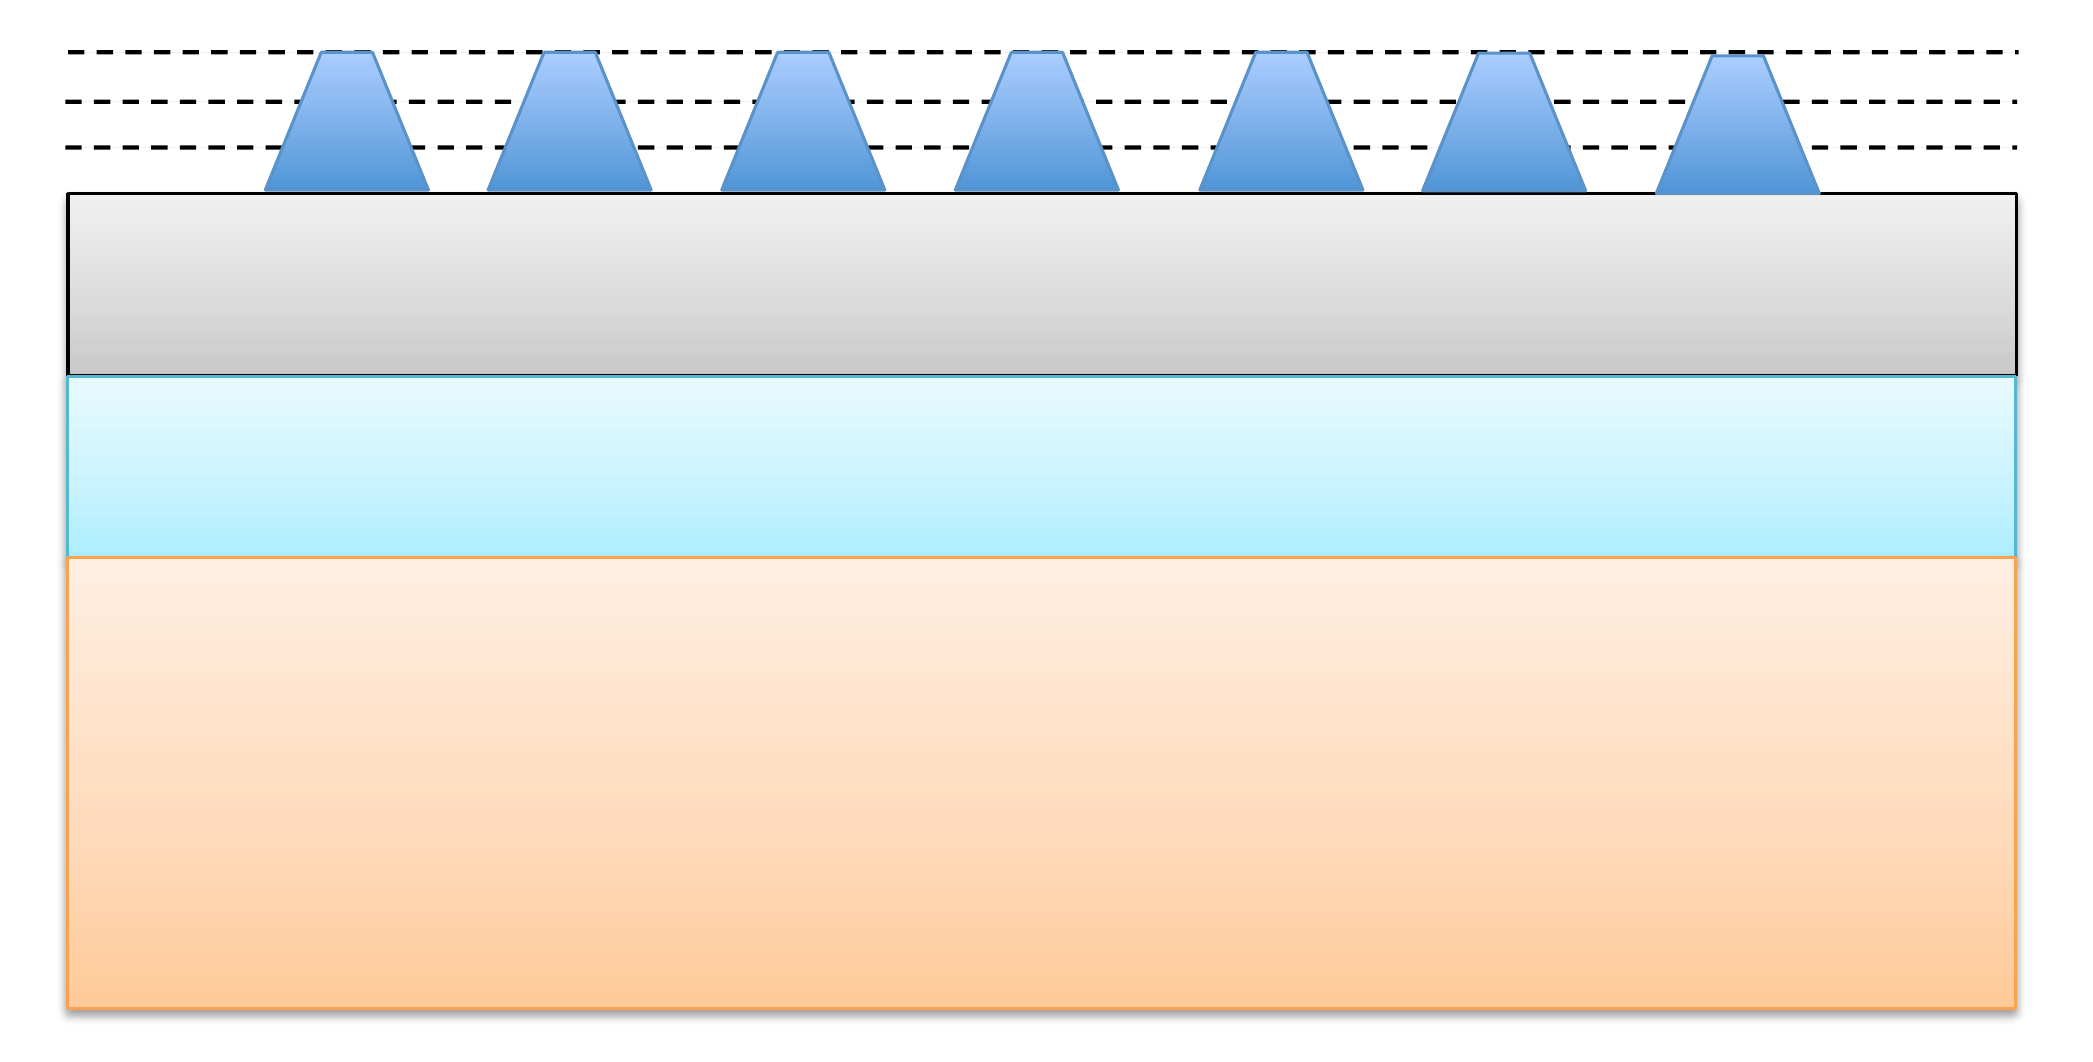
\includegraphics[width=8cm]{graded_layer.png}
        \\ Graded layer method
    \end{figure}
\end{frame}

\section{Interference functions}

\begin{frame}[fragile]
    \frametitle{Interference functions}
    \begin{center}
        See Jupyter notebook:\\
        \verb+interference_functions.ipynb+
    \end{center}
\end{frame}

\section{Roughness}

\begin{frame}[fragile]
    \frametitle{Rough interfaces}
    \begin{center}
        See Jupyter notebook:\\
        \verb+roughness.ipynb+
    \end{center}
\end{frame}

\end{document}